%%%%%%%%%%%%%%%%%%%%%%%%%%%%%%%%%%%%%%
%%  
%% Chapter 3: What is OpenMP
%%
%%%%%%%%%%%%%%%%%%%%%%%%%%%%%%%%%%%%%%

\def\ArtDir{03.Target/figures}%
 
\chapter{Running on a target device}
\label{chapter:target}

\section{Host/device model}
\begin{itemize}
  \item Host with target attached.
  \item Target has its own memory space.
  \item Can have more than one target, device() clause.
  \item Data moved between host and device by implicit rules and explicit directives.
\end{itemize}

When an OpenMP program begins running, it starts executing on the host processor.
This host processor is usually a CPU.
This initial thread is essentially the serial program that is running before any OpenMP directives are encountered.
The host processor has a memory space, which is shared between all threads running on the host processor.

Connected to this host are zero or more target devices. These target devices could be GPUs or other accelerators.
They each have their own memory space, which is distinct from the memory space of the host processor or any other device.
This means that data in our programs will be stored either in host memory or device memory.
OpenMP provides us with implicit rules for automatic data transfer along with explicit controls for the transfer of data between these memory spaces.
If the hardware supports it, OpenMP can also operate with a unified view of memory where the whole system sees a single memory space available to all; a topic we discuss in chapter~\ref{chapter:memory}.

In figure~\ref{fig:host_device} we show a host with three connected target devices.

\begin{figure}[t]
\label{fig:host_device}
\centerline{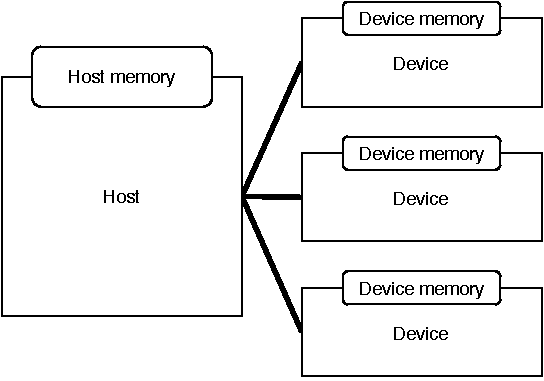
\includegraphics[width=200pt]{\ArtDir/host_device.pdf}}
\caption[The OpenMP host/device model consits of a host processor (typically a CPU) where execution begins, with zero or more attached target devices.
Data and execution can be offloaded from the host to the target device.
The memory spaces are distinct.]
{The OpenMP host/device model consists of a host processor (typically a CPU) where execution begins, with zero or more attached target devices.
Data and execution can be offloaded from the host to the target device.
The memory spaces are distinct.}
\end{figure}

We can query the OpenMP runtime for the number of available target devices in the system using the \texttt{omp\_get\_num\_devices()} API call.

\begin{verbatim}
#include <stdio.h>
#include <omp.h>

int main() {
  printf("There are %d devices\n",
    omp_get_num_devices());
}
\end{verbatim}

\subsection{Target construct offloading execution}
\begin{itemize}
  \item Target directive.
  \item Defines movement of execution to the target device.
  \item Host waits for the region to finish.
  \item Don't want too much detail on the tasking model here because will go into it in Chapter~\ref{chapter:async}. It's not relevant for getting starting this early on.
\end{itemize}

\section{The target memory environment and implicit mapping rules.}
\begin{itemize}
  \item target directive also triggers data movement as well as execution.
  \item first place where data movement is allowed, and will introduce the others at appropriate points.
  \item Different kinds of data we want to move: scalars, (stack) arrays, heap data/pointers, structures.
\end{itemize}

\subsection{Scalar variables}
\begin{itemize}
  \item Mapped as firstprivate.
  \item Example: {\tt int N; double x;}
  \item a scalar struct, as long as it is a complete type
  \item {\bf Not} copied back to the host at end of target region.
\end{itemize}

\subsection{Stack arrays}
\begin{itemize}
  \item Fixed sized stack arrays.
  \item Example: {\tt double arr[1024];}
  \item Complete types. Arrays of structs if complete type.
  \item Copied to device at start of target region, copied back at the end.
  \item Host not allowed to use copy in the meantime (with further details on this in Chapter~\ref{chapter:async}\dots).
  \item Data shared between {\bf all threads} on a device.
\end{itemize}

\subsection{Warning: heap arrays and pointers - reference later chapter}
\begin{itemize}
  \item We don't introduce the map clause yet.
  \item This is done in Chapter~\ref{chapter:memory}.
  \item This section says that we must do something explicit for everything not covered by the implicit rules.
  \item Examples of those would be heap arrays, and data-structures with pointers.
\end{itemize}

\section{Example: Vector add. arrays on stack. No need for map clauses yet.}
\begin{itemize}
  \item Takes vector add example from Chapter~\ref{chapter:overview}.
  \item Arrays are allocated on the stack, so follows implicit mapping rules.
  \item Example will simply transfer execution.
  \item Parallelism comes in Chapter~\ref{chapter:parallelism}.
  \item In OpenCL, have to deal with the host API copying buffers to/from host and device before we can run a meaningful kernel. Thinking in OpenCL might help here.
\end{itemize}

